

\chapter{Construction d'un heptadécagone régulier}\label{c.heptadecagon}

%%%%%%%%%%%%%%%%%%%%%%%%%%%%%%%%%%%%%%%%%%%%%%%%%%%%%%%%%%%%%%%



%%%%%%%%%%%%%%%%%%%%%%%%%%%%%%%%%%%%%%%%%%%%%%%%%%%%%%%%%%%%%%%

Les seuls polygones réguliers que les Grecs savaient construire à la  règle et au compas étaient le triangle, le carré, le pentagone et le polygone régulier à 15 côtés. À partir d'un polygone régulier à $n$  côtés, on peut construire un polygone à $2n$  côtés en circonscrivant le polygone par un cercle et en bissectant l'angle central (fig.~\ref{f.hept-double}). Aucun autre progrès n'a été réalisé jusqu'en 1796, lorsque Carl Friedrich Gauss s'est réveillé un matin, juste avant son 19$^\text{e}$  anniversaire, et a trouvé par une \og pensée concentrée\fg{} comment construire un heptadécagone régulier, un polygone régulier à 17  côtés. Cet exploit lui a donné envie de devenir mathématicien.

\begin{figure}[htbp]
\centering
\begin{tikzpicture}[scale=.5]
\coordinate (O) at (0,0);
\vertex{O};
\foreach \x/\name/\n/\po in {0/a/A/right,1/b/B/above,2/c/C/left,3/d/D/below left,4/e/E/below right} {
  \coordinate (\name) at ($(O)+(\x*72+18:3cm)$);
}
\draw (a) -- (b) -- (c) -- (d) -- (e) -- (a);
\node[draw,circle through=(a)] at (O) {};
\draw (d) -- (O) -- (e);
\draw [very thick,dotted] (O) -- (-90:3) -- (e) -- (-90:3) -- (d);
\end{tikzpicture}
%\includegraphics[width=0.5\textwidth]{Fig16_1}

\caption{Construction d'un polynôme régulier à 10 côtés à partir d'un pentagone régulier.}\label{f.hept-double}
\end{figure}

La section~\ref{s.hept-regular} traite de la relation entre le côté d'un polygone inscrit dans un cercle et l'angle central qu'il sous-tend. La section~\ref{s.fundamental} énonce sans démonstration le théorème fondamental de l'algèbre. La section~\ref{s.roots} présente les \emph{racines de l'unité}, les racines du polynôme $x^n-1$, qui sont au cœur de la démonstration de Gauss. Les sections~\ref{s.gauss} et~\ref{s.derivation} présentent la démonstration de Gauss qui est basée sur les symétries des racines des polynômes. Gauss a obtenu une formule qui montre que l'heptadécagone est constructible, mais aucune construction géométrique n'a été donnée pendant près d'un siècle. La section~\ref{s.construction} donne une construction élégante due à  James J. Callagy. La section~\ref{s.hept-pentagon} montre comment on peut construire un pentagone régulier en utilisant à la fois la géométrie et la trigonométrie.

Une partie du contenu est plus simple si on  la présente à l'aide de nombres complexes. Ces éléments sont présentés dans des encadrés qui peuvent être sautés.



\section{Construction des polygones réguliers}\label{s.hept-regular}

La construction de l'heptadécagone régulier a conduit au théorème de Gauss-Wantzel, qui stipule qu'un polygone régulier à $n$ côtés peut être construit à la règle et au  compas si et seulement si $n$ est le produit d'une puissance de $2$ et de zéro ou plusieurs nombres de Fermat distincts $2^{2^k}+1$ qui sont premiers. Les nombres premiers de Fermat connus sont 
\[
F_0=3,\quad F_1=5,\quad F_2=17,\quad F_3=257,\quad F_4=65\,537\,.
\]
Un polygone régulier à $257$ côtés a été construit par Magnus Georg Paucker en $1822$ et par Friedrich Julius Richelot en $1832$. En 1894, Johann Gustav Hermes a affirmé avoir construit un polygone régulier à 65\,537 côtés.

Pour construire un polygone régulier, il suffit de construire un segment  de longueur $\cos \theta$, où $\theta$ est l'angle central sous-tendu par une corde qui est un côté du polygone inscrit dans un cercle unité. Étant donné le segment $\overline{OB}=\cos\theta$, construisons une perpendiculaire à $B$. Soit $C$ son intersection avec le cercle unité. Alors 
\begin{align*}
\cos \theta&=\displaystyle\frac{\overline{OB}}{\overline{OC}}=\overline{OB}\,,\\
\theta &= \arccos (\overline{OB})\,.
\end{align*}
La corde $\overline{AC}$ est un côté du polygone régulier  (fig.~\ref{f.hept-central1}).

\begin{figure}[htbp]
\centering
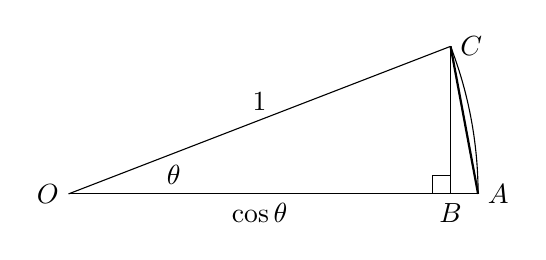
\begin{tikzpicture}[scale=1.3]
\coordinate (O) at (0,0) node[left] {$O$} node[above right,xshift=32pt] {$\theta$};
\coordinate (A) at (4,0);
\node[right] at (A) {$A$};
\draw (O) -- (A);
\draw (A) arc(0:21.12:4);
\coordinate (C) at (21.12:4cm);
\draw (O) -- node[above] {$1$} (C);
\node[right] at (C) {$C$};
\draw (C) -- (C |- A) coordinate (B);
\node[below] at (B) {$B$};
\draw[rotate=90] (B) rectangle +(5pt,5pt);
\draw[thick] (A) -- (C);
\path (O) -- node[below] {$\cos \theta$} (B); 
\end{tikzpicture}
%\includegraphics[width=0.7\textwidth]{Fig16_2}
\caption{Le cosinus de l'angle central d'un polygone régulier.}\label{f.hept-central1}
\end{figure}

Pour un segment de longueur $1$, les longueurs constructibles sont celles qui peuvent être obtenues à partir de segments de longueur connue en utilisant les opérations $\{+,-,\times,/,\surd\}$ (sect.~\ref{s.trisect-constructible}). Gauss a montré que $\cos(360^\circ/17)$, le cosinus de l'angle central d'un heptadécagone, est constructible puisqu'il peut être exprimé en utilisant uniquement ces opérations :
\begin{align*}
\cos\left(\frac{360^\circ}{17}\right) &= 
-\frac{1}{16}+\frac{1}{16}\sqrt{17} + 
     \frac{1}{16}\sqrt{34-2\sqrt{17}}
     \\
    &\quad
     +\frac{1}{8}\sqrt{
     17+3\sqrt{17} - 
     \sqrt{34-2\sqrt{17}}
   -2
     \sqrt{34+2\sqrt{17}}
   }\,.
\end{align*}

\section{Le théorème fondamental de l'algèbre}\label{s.fundamental}

Le théorème suivant sera utilisé sans démonstration.

\begin{theorem}\label{thm.fundamental} Tout polynôme de degré $n$ a exactement $n$ racines.
\end{theorem}

L'énoncé du théorème a été simplifié car tout ce dont nous aurons besoin est de savoir que $n$ racines existent.

\smallskip

\begin{advanced}
\textbf{Le théorème fondamental de l'algèbre} stipule que tout polynôme non constant de degré $n$ dans une seule variable avec des coefficients complexes a exactement $n$ racines complexes. 
S'il existe plusieurs racines ayant la même valeur, elles sont toutes comptées : $x^2-4x+4=(x-2)(x-2)$ a deux racines toutes deux égales à $2$.
Le polynôme $x^2+1$ à coefficients entiers a deux racines complexes $\pm\sqrt{-1}$.
Étrangement, même si le théorème concerne des entités algébriques finies -- des polynômes de degré $n$ avec $n$ racines -- des méthodes d'analyse, généralement l'analyse complexe, sont nécessaires pour démontrer le théorème.
\end{advanced}

\section{Les racines de l'unité}\label{s.roots}

D'après le théorème fondamental de l'algèbre (théorème~\ref{thm.fundamental}), le polynôme $x^{n}-1$ a $n$ racines pour tout entier $n> 1$. On observe que $x=1$ est une racine. Donc il y a $n-1$ autres racines. On désigne l'une de ces racines par $r$. Puisque $r^{n}=1$, la racine est appelée une \emph{racine $n$-ième de l'unité}. Qu'en est-il de $r^2$ ?
\[
(r^{2})^n=(r^{n})^2=1^2=1\,.
\]
Il s'ensuit que les $n$ nombres 
\[
1, r, r^2, \ldots, r^{n-2}, r^{n-1}
\]
sont des racines $n$-ième de l'unité.

\begin{advanced}
Soit $r=\cos \left(\frac{2\pi}{n}\right) + i\sin  \left(\frac{2\pi}{n}\right)$.
D'après la formule de Moivre,
\[
\left[\cos \left(\frac{2\pi}{n}\right) + i\sin  \left(\frac{2\pi}{n}\right)\right]^{n}=
\cos \left(\frac{2 n\pi}{n}\right) + i\sin  \left(\frac{2 n\pi}{n}\right)= 1\,.
\]
\vspace{-2ex}
\end{advanced}



\begin{theorem}
Soit $n$ un nombre premier et soit $r$ une racine $n$-ième  de l'unité. Alors 
\[
\{1,r,r^2,\ldots,r^{n-2},r^{n-1}\}
\]
sont distinctes, donc ce sont toutes les racines $n$-ièmes  de l'unité.
\end{theorem}

\begin{proof}
Supposons que les puissances ne soient pas distinctes de sorte que $r^i=r^j$ avec $0\leq i<j\leq n-1$. Alors $r^j/r^i=r^{j-i}=1$ donc il existe  un entier  $i'$ avec $0<i'<n$  tel que $r^{i'}=1$. Soit $m$ le plus petit de ces entiers strictement  positifs. Par l'algorithme de division euclidienne pour les entiers,  $n=ml+k$ avec $0<l<n$ et $0\leq k<m$. De 
\[
1=r^n=r^{ml+k}=(r^m)^l\cdot r^k=1^l\cdot r^k=r^k\,,
\]
on déduit $0\leq k<m$ et $r^k=1$. Puisque $m$ a été défini comme étant le plus petit entier strictement positif de ce type, $k=0$ et $n=ml$ n'est pas premier.
\end{proof}

\begin{theorem} Soit $\{a_1,a_2,\ldots,a_{n-1},a_n\}$ les racines d'un polynôme unitaire $f(x)$ de degré $n$. Alors 
\begin{align}\label{eq.viete}
f(x) =(x-a_1) (x-a_2)\cdots (x-a_{n-1})(x-a_n)\,.
\end{align}
\end{theorem}

\begin{proof}
Si $a_i$ est une racine de $f(x)$, on a par définition $f(a_i)=0$. La division euclidienne de $f(x)$ par $x-a_i$ donne  
\[
f(x)=(x-a_i)g_i(x)+f(a_i)=(x-a_i)g_i(x)\]
 pour un certain polynôme $g_i(x)$ de degré $n-1$. Le théorème résulte d'une  récurrence sur le degré.
\end{proof}

D'après l'équation~\ref{eq.viete} il est facile de voir que le coefficient de $x^{n-1}$ est 
\[
-(a_1+a_2+\cdots+a_{n-1}+a_n)\,.
\]
Puisque le coefficient de $x^{n-1}$ dans $x^n-1$ pour $n\geq 2$ est nul, on a 
\begin{align*}
-(1+r+r^2+\cdots + r^{n-2}+r^{n-1})&=0\,,\\
r+r^2+\cdots + r^{n-2}+r^{n-1}&=-1\,.
\end{align*}
Pour l'heptadécagone, on obtient
\begin{multline}
r+r^2+r^3+r^4+r^5+r^6+r^7+r^8+\\
r^9+r^{10}+r^{11}+r^{12}+r^{13}+r^{14} + r^{15}+r^{16}=-1.\label{eq.minus-one}
\end{multline}

\section{La démonstration de Gauss qu'un heptadécagone est constructible}\label{s.gauss}

Ce que Gauss a compris, c'est qu'il n'est pas nécessaire de travailler avec les racines dans leur ordre naturel $r,r^2,\ldots,r^{16}$. Les puissances de $3$ modulo 17 ($3^0$, $3^1$, $3^2$...) donnent toutes les racines mais dans un ordre différent :
\[
r^1, \;r^{1\cdot 3 =3},\; r^{3\cdot 3=9},\; r^{9\cdot 3=27=10},\; r^{10\cdot 3=30=13},\; r^{13\cdot 3=39=5},\; r^{5\cdot 3=15},\; r^{15\cdot 3=45=11},\]
\[
r^{11\cdot 3 =33=16}, \;r^{16\cdot 3=48=14},\; r^{14\cdot 3=42=8},\; r^{8\cdot 3=24=7},\;r^{7\cdot 3=21=4},\; r^{4\cdot 3=12},\; r^{12\cdot 3=36=2},\; \]
\[r^{2\cdot 3=6}\,,\]
où les racines ont été réduites modulo $17$ :
\[
r^{17m+k}=(r^{17})^m\cdot r^k=1^m\cdot r^k=r^k\,.
\]
Vérifions que la liste contient toutes les racines (sauf $1$) exactement une fois :
\begin{align}\label{eq.roots}
r^1, r^3, r^9, r^{10}, r^{13}, r^5, r^{15}, r^{11}, r^{16}, r^{14}, r^8, r^7, r^4, r^{12}, r^2, r^6\,.
\end{align}
Étant donné un polynôme unitaire du second degré  dont les racines sont $a$ et $b$,
\[
y^2+py+q=(y-a)(y-b)=0\,,
\]
on peut calculer les coefficients $p$ et $q$ à partir des racines 
 (chap.~\ref{c.quadratic}):
\[
p=-(a+b)\,,\quad q=ab\,.
\]
Par conséquent, étant donné $a+b$ et $ab$, nous pouvons écrire l'équation du second degré dont $a$ et $b$ sont les racines.

Soit $a_0$ la somme des racines dans les positions impaires de l'équation~\ref{eq.roots} :
\[
a_0=r + r^9 + r^{13} +r^{15} +r^{16} + r^8+r^4+r^2\,,
\]
et soit $a_1$ la somme des racines dans les positions paires de l'équation~\ref{eq.roots} :
\[
a_1=r^3 + r^{10} + r^{5} +r^{11} +r^{14} + r^7+r^{12}+r^6\,.
\]
Pour obtenir $a_0$ et $a_1$ comme racines d'une équation du second degré, il faut d'abord calculer leur somme et utiliser l'équation~\ref{eq.minus-one}:
\[
a_0+a_1=r + r^2 + \cdots +r^{16}=-1\,.
\]
Nous devons maintenant travailler  dur pour calculer leur produit. Dans le calcul, les valeurs de $r^ir^j=r^{i+j}$ sont écrites après réduction des exposants modulo $17$:
\[
\renewcommand{\arraystretch}{1.7}
\begin{array}{lcl}
a_0a_1&=&(r + r^9 + r^{13} +r^{15} +r^{16} + r^8+r^4+r^2)\;\;\times\\
&&(r^3 + r^{10} + r^{5} +r^{11} +r^{14} + r^7+r^{12}+r^6)\\
&=&\occ{4}{1} + \occ{11}{1} + \occ{6}{1} + \occ{12}{1} + \occ{15}{1} + \occ{8}{1} + \occ{13}{1} + \occ{7}{1} +\\
&&\occ{12}{2} + \occ{2}{1} + \occ{14}{1} + \occ{3}{1} + \occ{6}{2} + \occ{16}{1} + \occ{4}{2} + \occ{15}{2} +\\
&&\occ{16}{2} + \occ{6}{3} + \occ{1}{1} + \occ{7}{2} + \occ{10}{1} + \occ{3}{2} + \occ{8}{2} + \occ{2}{2}\;\;\: +\\
&&\occ{1}{2} + \occ{8}{3} + \occ{3}{3} + \occ{9}{1} + \occ{12}{3} + \occ{5}{1} + \occ{10}{2} + \occ{4}{3}\;\;\: +\\
&&\occ{2}{3} + \occ{9}{2} + \occ{4}{4} + \occ{10}{3} + \occ{13}{2} + \occ{6}{4} + \occ{11}{2} + \occ{5}{2} \:+\\
&&\occ{11}{3} + \occ{1}{3} + \occ{13}{3} + \occ{2}{4} + \occ{5}{3} + \occ{15}{3} + \occ{3}{4} + \occ{14}{2} \;+\\
&&\occ{7}{3} + \occ{14}{3} + \occ{9}{3} + \occ{15}{4} + \occ{1}{4} + \occ{11}{4} + \occ{16}{3} + \occ{10}{4} +\\
&&\occ{5}{4} + \occ{12}{4} + \occ{7}{4} + \occ{13}{4} + \occ{16}{4} + \occ{9}{4} + \occ{14}{4} + \occ{8}{4}\\
&=&-4\,.
\end{array}
\]
En effet, chaque racine apparaît exactement quatre fois et  l'équation \ref{eq.minus-one} montre que la valeur du produit est $-4$.


Puisque $a_0+a_1=-1$ et $a_0 a_1=-4$, $a_1$ et $a_2$ sont les racines de l'équation du second degré $y^2+y-4=0$. Elles peuvent être calculées en utilisant la formule pour les racines d'une équation du second degré\footnote{N.D.T. Il faut préciser comme dans \cite{Carrega} que $\theta=360^\circ/17$ implique $r+r^{16}=2\cos \theta>1$, $r^2+r^{15}=2\cos(2\theta)>1$,  $r^4+r^{13}=2\cos (4\theta)>0$ et $r^8+r^9=2\cos(8\theta)>-2$. Donc $a_0>0$.}:
\[
a_{0} = \frac{-1+\sqrt{17}}{2}\,,\quad a_{1} = \frac{-1-\sqrt{17}}{2}\,,
\]
Maintenant, soient $b_0,b_1,b_2,b_3$ les sommes d'une racine sur quatre à partir de $r^1,r^3,r^9,r^{10}$, respectivement :
\begin{align*}
b_0&= r^1+ r^{13} + r^{16} + r^4\,,\\
b_1&= r^3+ r^{5} + r^{14} + r^{12}\,,\\
b_2&= r^9+ r^{15} + r^{8} + r^2\,,\\
b_3&= r^{10}+ r^{11} + r^{7} + r^6\,.
\end{align*}
Vérifions que $b_0+b_2=a_0$ et $b_1+b_3=a_1$. Calculons les produits correspondants :
\begin{align*}
b_0b_2&=(r + r^{13} + r^{16} +r^4)\times (r^9 + r^{15} + r^{8} +r^{2})\\
&=(r^{10}+r^{16}+r^9+r^3)+(r^{5}+r^{11}+r^4+r^{15})+\\
&\quad \quad (r^{8}+r^{14}+r^7+r^1)+(r^{13}+r^{2}+r^{12}+r^6)\\
&=-1\,,\\
b_1b_3&=(r^3 + r^{5} + r^{14} +r^{12})\;\;\times\;(r^{10} + r^{11} + r^{7} +r^{6})\\
&=(r^{13}+r^{14}+r^{10}+r^9)+(r^{15}+r^{16}+r^{12}+r^{11})+\\
&\quad \quad (r^{7}+r^{8}+r^4+r^3) +(r^{5}+r^{6}+r^{2}+r^1)\\
&=-1\,.
\end{align*}
Pour résumer ces calculs :
\begin{align*}
b_0+b_2&=a_0\,,\\
b_0b_2&=-1\,,\\
b_1+b_3&=a_1\,,\\
b_1b_3&=-1\,.
\end{align*}
Donc $b_0$ et $b_2$ sont les solutions de $y^2-a_0y-1= 0$, tandis que $b_1$ et $b_3$ sont les solutions de $y^2-a_1y-1 =0$. En utilisant les valeurs calculées précédemment pour $a_0$ et $a_1$, nous pouvons calculer\footnote{N.D.T. On a $r+r^{16}=2\cos \theta>2\cos(2\theta)=r^2+r^{15}$ et $r^4+r^{13}=2\cos (4\theta)>2\cos(8\theta)$. Donc $b_0>b_2$. De même, $b_1>b_3$.} les racines $b_0$ et $b_1$:
\begin{align*}
b_0&=\frac{a_0+\sqrt{a_0^2+4}}{2}\\
&=\frac{
     \displaystyle\frac{(-1+\sqrt{17})}{2} + 
     \sqrt{\left(\displaystyle\frac{(-1+\sqrt{17})}{2}\right)^2+4}
   }{2}\\
&=\frac{
     (-1+\sqrt{17}) + 
     \sqrt{\left(-1+\sqrt{17}\right)^2+16}
   }{4}\\
&=\frac{
     (-1+\sqrt{17}) + 
     \sqrt{34-2\sqrt{17}}
   }{4}\,,\\
b_1&=\frac{a_1+\sqrt{a_1^2+4}}{2}\\
&=\frac{
     \displaystyle\frac{(-1-\sqrt{17})}{2} + 
     \sqrt{\left(\displaystyle\frac{(-1-\sqrt{17})}{2}\right)^2+4}
   }{2}\\
&=\frac{
     (-1-\sqrt{17}) + 
     \sqrt{\left(-1-\sqrt{17}\right)^2+16}
   }{4}\\
&=\frac{
     (-1-\sqrt{17}) + 
     \sqrt{34+2\sqrt{17}}
   }{4}\,.
\end{align*}

Enfin, soient $c_0$ et $c_4$ les sommes d'une racine sur huit en commençant par $r^1$ et $r^{13}$ :
\begin{align*}
c_0&=r^1+r^{16}\,,\\
c_4&=r^{13}+r^4\,,\\
c_0+c_4&=r^1+r^{16}+r^{13}+r^4=b_0\,,\\
c_0c_4&=(r^1+r^{16})\cdot(r^{13}+r^4)\\
&=r^{14}+r^5+r^{12}+r^3=b_1\,.
\end{align*}
Donc $c_0$ et $c_4$ sont les racines de $y^2-b_0y+b_1=0$. Puisque $\cos(360^\circ/17) = c_0/2$ (fig.~\ref{f.hept-cosine} et encadré), il suffit de calculer\footnote{N.D.T. On a $c_0=2\cos \theta>2\cos(4\theta)=c_4$.} la racine $c_0=r^1+r^{16}$:
\begin{align*}
c_0&=\frac{b_0+\sqrt{b_0^2-4b_1}}{2}\\
&=\frac{1}{2}
     \frac{
     (-1+\sqrt{17}) + 
     \sqrt{34-2\sqrt{17}}
   }{4} \\
&\quad  +
    \frac{1}{2}
       \sqrt{\left(\frac{
     (-1+\sqrt{17}) + 
     \sqrt{34-2\sqrt{17}}
   }{4}\right)^2-4\left(\frac{
     (-1-\sqrt{17}) + 
     \sqrt{34+2\sqrt{17}}
   }{4}\right)}
   \\
&=-\frac{1}{8}+\frac{1}{8}\sqrt{17} + 
     \frac{1}{8}\sqrt{34-2\sqrt{17}}
     \\
   &\quad + 
     \frac{1}{8}\sqrt{
     \left(
     (-1+\sqrt{17}) + 
     \sqrt{34-2\sqrt{17}}
   \right)^2-16\left(
     (-1-\sqrt{17}) + 
     \sqrt{34+2\sqrt{17}}
   \right)}
\\
&=-\frac{1}{8}+\frac{1}{8}\sqrt{17} + 
     \frac{1}{8}\sqrt{34-2\sqrt{17}}
    \\
   &\quad +
     \frac{1}{8}\sqrt{
     (-1+\sqrt{17})^2 + 
     2(-1+\sqrt{17})\sqrt{34-2\sqrt{17}}+
     (34-2\sqrt{17})
   -}\\
   &\quad \overline{
     \left((-16-16\sqrt{17}) + 
     16\sqrt{34+2\sqrt{17}}\right)
   }
\\
&=-\frac{1}{8}+\frac{1}{8}\sqrt{17} + 
     \frac{1}{8}\sqrt{34-2\sqrt{17}}
     \\
   &\quad +
     \frac{1}{8}\sqrt{
     68+12\sqrt{17} + 
     2(-1+\sqrt{17})\sqrt{34-2\sqrt{17}}
   -16
     \sqrt{34+2\sqrt{17}}
   }
\end{align*}

\begin{figure}[htbp]

\centering
\begin{tikzpicture}[scale=1]
\coordinate (O) at (0,0) node[left] {$O$}
  node[above right,xshift=20pt] {$\theta$}
  node[below right,xshift=20pt] {$\theta$};
\coordinate (A) at (4,0);
\coordinate (C) at (21.12:4cm);
\coordinate (D) at (-21.12:4cm);
\draw (D) arc(-21.12:21.12:4);
\draw (D) -- node[below] {$1$} (O) -- node[above] {$1$} (C);
\node[right] at (C) {$r^1$};
\node[right] at (D) {$r^{16}$};
\draw (C) -- (C |- A) coordinate (B);
\draw (D) -- (D |- A);
\draw[rotate=90] (B) rectangle +(5pt,5pt);
\draw (D) -- (A) -- (C);
\draw[<->] ($(O)+(3pt,0)$) --
  node[fill=white] {$\cos \theta$} (B);
\end{tikzpicture}
%\includegraphics[width=0.6\textwidth]{Fig16_5}

\caption{Le cosinus de l'angle central calculé à partir de $r_1$ et $r_{16}$.}\label{f.hept-cosine}
\end{figure}

Le cosinus de l'angle central d'un heptadécagone est constructible à la  règle et au compas puisqu'il n'est composé que de nombres rationnels et des opérations $\{+,-,\times,/,\surd\}$:
\begin{flalign}
\cos\left(\frac{360^\circ}{17}\right) &= 
\frac{c_0}{2}\\
&=-\frac{1}{16}+\frac{1}{16}\sqrt{17} + 
     \frac{1}{16}\sqrt{34-2\sqrt{17}}\; +
    \label{eq.not-gauss1}\\
 & \quad\frac{1}{16}\sqrt{
     68+12\sqrt{17} + 
     2(-1+\sqrt{17})\sqrt{34-2\sqrt{17}}
   -16
     \sqrt{34+2\sqrt{17}}
   }\,.\label{eq.not-gauss2}
\end{flalign}


\begin{advanced}
\vspace{-4ex}
\begin{eqnarray*}
r_1+r_{16}&=&\cos\left(\frac{2\pi}{17}\right)+i\sin\left(\frac{2\pi}{17}\right)+\cos\left(\frac{2\cdot 16\pi}{17}\right)+i\sin\left(\frac{2\cdot 16\pi}{17}\right)\\
&=&\cos\left(\frac{2\pi}{17}\right)+i\sin\left(\frac{2\pi}{17}\right)+\cos\left(\frac{-2\pi}{17}\right)+i\sin\left(\frac{-2\pi}{17}\right)\\
&=&2\cos\left(\frac{2\pi}{17}\right)\,.
\end{eqnarray*}
\vspace{-6ex}
\end{advanced}

\section{Démonstration de la formule de Gauss}\label{s.derivation}

La formule ci-dessus pour $\cos(360^\circ /17)$ n'est pas celle donnée par Gauss. Voici une démonstration de la formule de Gauss.

Simplifions $2(-1+\sqrt{17})\sqrt{34-2\sqrt{17}}$:
\begin{align*}
2(-1+\sqrt{17})\sqrt{34-2\sqrt{17}} &=
-2\sqrt{34-2\sqrt{17}} +2\sqrt{17}\sqrt{34-2\sqrt{17}}\\
&\quad \quad +4\sqrt{34-2\sqrt{17}}-4\sqrt{34-2\sqrt{17}}\\
&=
2\sqrt{34-2\sqrt{17}} +2\sqrt{17}\sqrt{34-2\sqrt{17}}\\
&\quad \quad -4\sqrt{34-2\sqrt{17}}\\
&=2(1+\sqrt{17})\sqrt{34-2\sqrt{17}}-4\sqrt{34-2\sqrt{17}}\,.
\end{align*}
Nous nous souviendrons du terme $-4\sqrt{34-2\sqrt{17}}$  et simplifierons le premier terme en le mettant au carré puis en prenant la racine carrée :
\begin{align*}
2(1+\sqrt{17})\sqrt{34-2\sqrt{17}}&=
2\sqrt{\left[(1+\sqrt{17})\sqrt{34-2\sqrt{17}}\right]^2}\\
&=2\sqrt{(18+2\sqrt{17})(34-2\sqrt{17})}\\
&=2\sqrt{(18\cdot 34-4\cdot17)+\sqrt{17}(2\cdot 34 - 2\cdot 18)}\\
&=2\cdot 4\sqrt{34+2\sqrt{17}}\,.
\end{align*}
En substituant les termes, on obtient la formule de Gauss :
\begin{align*}
&\cos\left(\frac{360^\circ}{17}\right) \\
&=
-\frac{1}{16}+\frac{1}{16}\sqrt{17} + 
     \frac{1}{16}\sqrt{34-2\sqrt{17}} \\
    &
     \quad +\frac{1}{16}\sqrt{
     68+12\sqrt{17} + 
     8\sqrt{34+2\sqrt{17}}-4\sqrt{34-2\sqrt{17}}
   -16
     \sqrt{34+2\sqrt{17}}
   }\\
&=-\frac{1}{16}+\frac{1}{16}\sqrt{17} + 
     \frac{1}{16}\sqrt{34-2\sqrt{17}}\\
&\quad +\frac{1}{8}\sqrt{
     17+3\sqrt{17} - 
     \sqrt{34-2\sqrt{17}}
   -2
     \sqrt{34+2\sqrt{17}}
   }\,.
\end{align*}

\section{Construction d'un heptadécagone}\label{s.construction}

Construisons un cercle unité de centre $O$ avec des diamètres perpendiculaires $\overline{QP}$ et $\overline{SR}$  (fig.~\ref{f.hept-construction1}).
\begin{figure}[htbp]
\centering
        \begin{tikzpicture}[scale=1.2]
\clip (-4.3,-1.8) rectangle (4.3,1.9);

\node at (-.2,1.5) {$\cdots$};
\node at (-.2,1.7) {$R$};
\node at (-.2,-1.5) {$\cdots$};
\node at (-.2,-1.7) {$S$};

\coordinate (O) at (0,0);
\draw (O) circle (4cm);
\coordinate (P) at (4,0);
\coordinate (R) at (0,4);
\coordinate (Q) at (-4,0);
\coordinate (S) at (0,-4);
\coordinate (A) at (0,1);
\coordinate (B) at (.78,0);
\coordinate (C) at (-1.28,0);
\draw (P) -- (Q);
\draw (R) -- (S);
\path (O) -- node[left,xshift=2pt,yshift=-4pt] {$\frac{1}{4}$} (A);
\draw (P) -- ($(P)!1.5!(A)$);
\draw (A) -- node[above] {$\frac{\sqrt{17}}{4}$} (P);
\draw (C) -- (A) -- (B);
\foreach \c/\where in {O/below left, P/right, Q/left, R/above, S/below, A/above left, B/below, C/below} {
  \node[\where] at (\c) {$\c$};
}
\draw (O) rectangle(+5pt,+5pt);
%\vertex{O};
\node[below right,xshift=8pt,yshift=-4pt] at (A) {\sm{\alpha}};
\node[below right,xshift=-2pt,yshift=-6pt] at (A) {\sm{\alpha}};
\node[below left,xshift=1pt,yshift=-2pt] at (A) {\sm{\beta}};
\node[below left,xshift=-4pt,yshift=3pt] at (A) {\sm{\beta}};
\draw[<->] ($(C)+(0,-16pt)$) -- node[below] {$\frac{1+\sqrt{17}}{16}$} ($(O)+(0,-16pt)$);
\draw[<->] ($(O)+(0,-16pt)$) -- node[below,xshift=4pt] {$
\frac{-1+\sqrt{17}}{16}$} ($(B)+(0,-16pt)$);
\end{tikzpicture}
%\includegraphics[width=\textwidth]{Fig16_7}

\caption{Construction d'un heptadécagone 
 (1).}\label{f.hept-construction1}
\end{figure}
Construisons $A$ de sorte que $\overline{OA}=(1/4)\overline{OR}$.

D'après le théorème de Pythagore,
\[
\overline{AP}=\sqrt{\overline{OA}^2+\overline{OP}^2}=\sqrt{(1/4)^2+1^2}=\sqrt{17}/4\,.
\]
Soit $B$ l'intersection de la bissectrice interne de $\angle OAP$ et du segment  $\overline{OP}$. Soit $C$ l'intersection de la bissectrice externe de $\angle OAP$ et du segment $\overline{QO}$. D'après le théorème~\ref{thm.angle-bisector},
\begin{align*}
\frac{\overline{OB}}{\overline{BP}}&=\frac{\overline{AO}}{\overline{AP}}\,,\\
\frac{\overline{OB}}{1-\overline{OB}}&=\frac{1/4}{\sqrt{17}/{4}}\,,\\
\overline{OB}&=\frac{1}{1+\sqrt{17}}=\frac{1}{1+\sqrt{17}}\cdot \frac{1-\sqrt{17}}{1-\sqrt{17}}\\
&=\frac{-1+\sqrt{17}}{16}\,.
\end{align*}
D'après le théorème~\ref{thm.external-angle-bisector},
\begin{align*}
\frac{\overline{OC}}{\overline{CP}}&=\frac{\overline{AO}}{\overline{AP}}\,,\\
\frac{\overline{OC}}{1+\overline{OC}}&=\frac{1/4}{\sqrt{17}/{4}}\,,\\
\overline{OC}&=\frac{1}{-1+\sqrt{17}}=\frac{1}{-1+\sqrt{17}}\cdot \frac{1+\sqrt{17}}{1+\sqrt{17}}\\
&=\frac{1+\sqrt{17}}{16}\,.
\end{align*}
Construisons $D$ sur $\overline{OP}$ tel que 
 $\overline{CD}=\overline{CA}=a$ (figure~\ref{f.hept-construction2}). D'après le théorème de Pythagore,
\begin{align*}
\overline{CD}=\overline{CA}&=\sqrt{\overline{OA}^2+\overline{OC}^2}\\
&=\sqrt{\left(\frac{1}{4}\right)^2+\left(\frac{1+\sqrt{17}}{16}\right)^2}=\frac{1}{16}\sqrt{16+1+17+2\sqrt{17}}\\
&=\frac{1}{16}\sqrt{34+2\sqrt{17}}\,.
\end{align*}


\begin{figure}[htbp]
\centering
        \begin{tikzpicture}[scale=1.2]
\clip (-4.3,-1.8) rectangle (4.3,1.9);
\coordinate (O) at (0,0);
\draw (O) circle (4cm);
\coordinate (P) at (4,0);
\coordinate (R) at (0,4);
\coordinate (Q) at (-4,0);
\coordinate (S) at (0,-4);
\coordinate (A) at (0,1);
\coordinate (B) at (.78,0);
\coordinate (C) at (-1.28,0);

\coordinate (D) at (.344,0);
\coordinate (E) at (2.05,0);
\coordinate (M) at (-1.8275,0);
\coordinate (F) at (0,-1);

\draw (P) -- (Q);
\draw (R) -- (S);
\draw (A) -- (P);
\draw (C) -- node[above] {$a$} (A) -- node[xshift=2pt,right] {$b$} (B);
\path (Q) -- node[below] {$f$}  (M);
\path (B) -- node[below] {$b$} (E);

\path[name path=circ] (M) circle (2.1725cm);
\path[name path=yaxis] (R) -- (S);
\path[name intersections={of=circ and yaxis,by={F1,F}}];
\draw (M) -- node[below] {$f$} (F);

\draw[<->] ($(C)+(0,-9pt)$) -- node[fill=white] {$a$} ($(D)+(0,-9pt)$);

\foreach \c/\where in {O/below left, P/right, Q/left, R/above, S/below, A/above left, B/below, C/below, D/below, E/below, M/below left, F/below left} {
  \node[\where] at (\c) {$\c$};
}
\draw (O) rectangle(+5pt,+5pt);
%\vertex{O};
\vertex{E};
\vertex{D};
\end{tikzpicture}
%\includegraphics[width=\textwidth]{Fig16_8}

\caption{Construction d'un heptadécagone (2).}\label{f.hept-construction2}
\end{figure}



Construisons $E$ sur $\overline{OP}$ tel que $\overline{BE}=\overline{BA}=b$. Toujours d'après le théorème de Pythagore,
\begin{align*}
\overline{BE}=\overline{BA}&=\sqrt{\overline{OA}^2+\overline{OB}^2}\\
&=\sqrt{\left(\frac{1}{4}\right)^2+\left(\frac{-1+\sqrt{17}}{16}\right)^2}=\frac{1}{16}\sqrt{16+1+17-2\sqrt{17}}\\
&=\frac{1}{16}\sqrt{34-2\sqrt{17}}\,.
\end{align*}
Construisons le milieu $M$ de $\overline{QD}$ et construisons $F$ sur $\overline{OS}$ tel que 
 $\overline{MF}=\overline{MQ}=f$:
%
\begin{align*}
\overline{MF}=\overline{MQ}&=\frac{1}{2}\overline{QD}=\frac{1}{2}(\overline{QC}+\overline{CD})=\frac{1}{2}((1-\overline{OC})+\overline{CD})\\
&=\frac{1}{2}\left[1-\left(\frac{1+\sqrt{17}}{16}\right)+\frac{\sqrt{34+2\sqrt{17}}}{16}\right]\\
&=\frac{1}{32}\left(15-\sqrt{17}+\sqrt{34+2\sqrt{17}}\right)\,.
\end{align*}
Remarquons que $\overline{MO}=1-\overline{MQ}=1-\overline{MF}$.
 
\begin{figure}[htbp]
\centering
        \begin{tikzpicture}[scale=1.2]
\clip (-4.3,-1.8) rectangle (4.3,1.9);
\coordinate (O) at (0,0);
\draw (O) circle (4cm);
\coordinate (P) at (4,0);
\coordinate (R) at (0,4);
\coordinate (Q) at (-4,0);
\coordinate (S) at (0,-4);
\coordinate (A) at (0,1);
\coordinate (B) at (.78,0);
\coordinate (C) at (-1.28,0);

\coordinate (D) at (.5,0);
\coordinate (E) at (2.045,0);
\coordinate (M) at (-1.8275,0);

\path[name path=circ] (M) circle (2.1725cm);
\path[name path=yaxis] (R) -- (S);
\path[name intersections={of=circ and yaxis,by={F1,F}}];
\draw (M) -- node[below] {$f$} (F);

\draw[name path=OEarc] (E) arc(0:-180:1.025cm);
\path[name path=OFcircle] (O)
  let
    \p1 = ($(O)-(F)$)
  in
    circle({veclen(\x1,\y1)});
\path[name intersections={of=OEarc and OFcircle, by={G}}];
\draw (O) -- node[above,near end,xshift=2pt] {$g$} (G) -- node[below] {$e$} (E);
\path (O) -- node[left] {$g$} (F);

\path[name path=EGcircle] (E) 
  let
  \p1 = ($(E)-(G)$)
  in
    circle({veclen(\x1,\y1)});
\draw[name path=PQ] (P) -- (Q);
\path[name intersections={of=PQ and EGcircle, by={H,H1}}];
\path (E) -- node[below] {$e$} (H);

\draw (R) -- (S);
\draw (A) -- (P);
\draw (C) -- (A) -- (B);
\draw (M) -- (F);

\foreach \c/\where in {O/below left, P/right, Q/left, R/above, S/below, A/above left, B/below, C/below, D/below, E/below right, M/below left, F/below left, G/below, H/below} {
  \node[\where] at (\c) {$\c$};
}
%\vertex{O};
\vertex{D};
\vertex{H};
\draw (O) rectangle +(+5pt,+5pt);
\draw[rotate=30] (G) rectangle +(+5pt,+5pt);
\path (Q) -- node[below] {$f$} (M);
\end{tikzpicture}
%\includegraphics[width=\textwidth]{Fig16_9}

\caption{Construction d'un heptadécagone (3).}\label{f.hept-construction3}
\end{figure}


Construisons un demi-cercle dont le diamètre est $\overline{OE}$. Construisons une corde $\overline{OG}=\overline{OF}=g$ (fig.~\ref{f.hept-construction3}). D'après le théorème de Pythagore,
\begin{align*}
\overline{OG}=\overline{OF}&=\sqrt{\overline{MF}^2-\overline{MO}^2}=\sqrt{\overline{MF}^2-(1-\overline{MF})^2}\\
&=\sqrt{2\overline{MF}-1}\\
&=\sqrt{\frac{1}{16}\left(15-\sqrt{17}+\sqrt{34+2\sqrt{17}}\right)-1}\\
&=\frac{1}{4}\sqrt{-1-\sqrt{17}+\sqrt{34+2\sqrt{17}}}\,.
\end{align*}
$\angle OGE$ est un angle droit puisqu'il est sous-tendu par un diamètre du cercle. Construisons $H$ sur $\overline{OP}$ tel que $\overline{EH}=\overline{EG}=e$. Toujours d'après le théorème de Pythagore,
\begin{align*}
\overline{EH}=\overline{EG}&=\sqrt{\overline{OE}^2-\overline{OG}^2}=\sqrt{(\overline{OB}+\overline{BE})^2-\overline{OG}^2}\\
&=\sqrt{\left(\frac{-1+\sqrt{17}}{16}+\frac{\sqrt{34-2\sqrt{17}}}{16}\right)^2-
\frac{1}{16}\left(-1-\sqrt{17}+\sqrt{34+2\sqrt{17}}\right)}
\\
&=\frac{1}{16}\sqrt{\left(
(18-2\sqrt{17})+ 2(-1+\sqrt{17})\sqrt{34-2\sqrt{17}}+
(34-2\sqrt{17})\right)}\\
&\quad\quad\quad\overline{
+\left(16+16\sqrt{17}-16\sqrt{34+2\sqrt{17}}\right)}\\
&=\frac{1}{16}\sqrt{
68+12\sqrt{17}-16\sqrt{34+2\sqrt{17}}-2(1-\sqrt{17})\sqrt{34-2\sqrt{17}}
}\,.
\end{align*}


Calculons $\overline{OE}$:
\begin{align*}
\overline{OE}=\overline{OB}+\overline{BE}&=\frac{-1+\sqrt{17}}{16}+\frac{1}{16}\sqrt{34-2\sqrt{17}}\\
&=\frac{1}{16}\left(-1+\sqrt{17}+\sqrt{34-2\sqrt{17}}\right)\,.
\end{align*}
Enfin, $\overline{OH}=\overline{OE}+\overline{EH}$ qui est la formule de Gauss pour $\cos (360^\circ/17)$.



\section{Construction d'un pentagone régulier}\label{s.hept-pentagon}


\begin{advanced}
Les racines cinquièmes complexes de l'unité sont 
\[
1+i\cdot 0,\quad\frac{\sqrt{5}-1}{4}\pm i \frac{\sqrt{10+2\sqrt{5}}}{4},\quad\frac{-\sqrt{5}-1}{4}\pm i \frac{\sqrt{10-2\sqrt{5}}}{4}\,.
\]
\vspace{-3ex}
\end{advanced}

\subsection{Trigonométrie}
L'angle central d'un pentagone régulier est  $360^\circ/5=72^\circ$. Calculons $\cos 36^\circ$ en utilisant les formules trigonométriques pour $2\theta$ et $\theta/2$  (théorèmes~\ref{s.sum-of-trig} et \ref{thm.sine-cosine-half}):
\begin{align*}
0=\cos 90^\circ &= \cos(72^\circ+18^\circ)\\
&=\cos (2\cdot 36^\circ)\cos (36^\circ/2) - \sin (2\cdot 36^\circ)\sin (36^\circ/2)\\
&=(2\cos^2 36^\circ-1)\sqrt{\frac{1+\cos 36^\circ}{2}}-2\sin 36^\circ\cos 36^\circ\sqrt{\frac{1-\cos 36^\circ}{2}}\,.
\end{align*}
Il n'y a maintenant qu'un seul angle dans la formule. Soit $x=\cos 36^\circ$. Alors 
\begin{align*}
(2x^2-1)\sqrt{\frac{1+x}{2}}&=2\sqrt{1-x^2}\cdot x \cdot \sqrt{\frac{1-x}{2}}\,,\\
(2x^2-1)\sqrt{1+x}&=2\sqrt{1-x}\cdot\sqrt{1+x}\cdot x \cdot \sqrt{1-x}\,,\\
2x^2-1&=2x(1-x)\,,\\
4x^2-2x-1&=0\,.
\end{align*}
La résolution de l'équation du second degré donne une valeur constructible :
\[
\cos 36^\circ = \frac{1+\sqrt{5}}{4}\,.
\]

\subsection{Géométrie}\label{s.geometry-pentagon}

Soit $\overline{ABCDE}$ un pentagone régulier (fig.~\ref{f.hept-pentagon2}). Par définition, tous les côtés et tous les angles intérieurs sont égaux. Il est facile de montrer par des triangles isométriques que toutes les diagonales sont égales. Soit 1 la longueur des côtés. Soit $x$ la longueur des diagonales.

\begin{figure}[htbp]
\centering
        \begin{tikzpicture}[scale=.8]
\coordinate (O) at (0,0);
\vertex{O};
\node[above left,xshift=1pt,yshift=4pt] at (O) {$O$};
\foreach \x/\name/\n/\po in {0/a/A/right,1/b/B/above,2/c/C/left,3/d/D/below left,4/e/E/below right} {
  \coordinate (\name) at ($(O)+(\x*72+18:3cm)$);
  \node[\po] at (\name) {$\n$};
}
\draw (a) -- node[above] {$1$} (b) -- node[above] {$1$} (c) -- node[left] {$1$} (d) -- node[below] {$1$} (e) -- node[right] {$1$} (a);
\draw[thick] (a) -- node[above] {$x$} (c);
\draw[thick,name path=ad] (a) -- node[above] {$x$} (d);
\draw[thick,name path=cd] (c) -- node[above] {$x$} (e);
\path[name intersections={of=ad and cd,by={f}}];
\node[above] at (f) {$\psi$};
\vertex{f};
\node[below] at (f) {$\psi$};
\node[right,xshift=6pt] at (f) {$F$};
\node[below right,xshift=14pt] at (c) {$\theta$};
\node[below left,xshift=-14pt] at (a) {$\theta$};
\node[above right,xshift=16pt] at (d) {$\phi$};
\node[above left,xshift=-16pt] at (e) {$\phi$};
\end{tikzpicture}
%\includegraphics[width=0.6\textwidth]{Fig16_10}

\caption{Construction d'un pentagone régulier 
 (1).}\label{f.hept-pentagon2}
\end{figure}
$\triangle ACE\cong \triangle CAD$ (trois côtés égaux) donc $\angle ACE=\angle CAD=\theta$. $\triangle AED\cong\triangle CDE$  (trois côtés égaux) donc  $\angle ADE=\angle CED=\phi$. $\angle AFC=\angle EFD=\psi$ sont des angles opposés par le sommet. Dans les deux triangles, la somme des angles est  $180^\circ$, donc
$\psi+2\theta=\psi+ 2\phi$ et $\theta=\phi$.
Avec les angles alternes-internes, nous concluons que $\overline{AC}\parallel \overline{DE}$.

Construisons une droite qui passe  par $E$ et parallèle à $\overline{DC}$. Soit $F$ son intersection avec $\overline{AC}$ (fig.~\ref{f.hept-pentagon3}). $\overline{CDEF}$ est un losange,  donc $\overline{EF}=\overline{CD}=\overline{AE}=1$. $\triangle ACE$ est un triangle isocèle dont les angles de base sont $\alpha$. $\triangle AEF$ est également isocèle et $\angle AFE=\angle FAE=\alpha$, donc $\triangle ACE\sim \triangle AEF$. En prenant les rapports des côtés, on obtient
\[
\frac{x}{1}=\frac{1}{x-1}\,.
\]
Le résultat est une équation du second degré $x^2-x-1=0$ 
dont la racine positive est constructible :
\[
x=\frac{1+\sqrt{5}}{2}\,.
\]

\begin{figure}[htbp]
\centering
        \begin{tikzpicture}[scale=.8]
\coordinate (O) at (0,0);
\vertex{O};
\node[above left,xshift=1pt,yshift=4pt] at (O) {$O$};

\foreach \x/\name/\n/\po in {0/a/A/right,1/b/B/above,2/c/C/left,3/d/D/below left,4/e/E/below right} {
  \coordinate (\name) at ($(O)+(\x*72+18:3cm)$);
  \node[\po] at (\name) {$\n$};
}
\draw (a) -- node[above] {$1$} (b) -- node[above] {$1$} (c) -- node[left] {$1$} (d) -- node[below] {$1$} (e);
\draw[very thick] (e)-- node[right] {$1$} (a);
\draw[very thick] (a) -- (c);
\draw[very thick] (c) -- node[below] {$x$} (e);

\path[name path=ef] (e) -- +(108:5);
\path[name path=ac] (a) -- (c);
\path[name intersections={of=ac and ef,by={f}}];
\vertex{f};
\node[above] at (f) {$F$};
\draw[very thick] (e) -- node[right] {$1$} (f);
\path (a) -- node[above,xshift=-4pt] {$x-1$} (f);
\node[below left] at (a) {$\alpha$};
\node[below right,xshift=2pt] at (f) {$\alpha$};
\path (c) -- node[above] {$1$} (f);
\draw ($(e)+(72:.5)$) arc(72:144:.5cm);
\node[above,yshift=12pt] at (e) {$\alpha$};
\end{tikzpicture}
%\includegraphics[width=0.6\textwidth]{Fig16_11}

\caption{Construction d'un pentagone régulier 
 (2).}\label{f.hept-pentagon3}
\end{figure}

\subsection*{Quelle est la surprise ?}

Il est surprenant que deux millénaires se soient écoulés entre les travaux des Grecs  et la découverte par Gauss de la constructibilité de l'heptadécagone régulier. Il est également surprenant que le problème ait été résolu non pas en utilisant la géométrie mais en inventant de nouvelles méthodes algébriques qui ont eu une influence considérable sur les mathématiques.


\subsection*{Sources}

Ce chapitre se base sur \cite{jorg}. L'œuvre originale de Gauss est disponible dans une traduction française \cite{gauss}.
L'équation~\ref{eq.not-gauss1}--\ref{eq.not-gauss2} apparaît dans \cite{rike} ; l'auteur propose un exercice pour la transformer en la formule de Gauss telle qu'elle apparaît dans \cite[p.~458]{gauss} et \cite[p.~68]{jorg}.

La construction de l'heptadécagone est tirée de \cite{callagy} tandis que d'autres constructions peuvent être trouvées dans \cite{wiki:heptadecagon}. La construction trigonométrique du pentagone régulier est tirée de \cite{wiki:pentagon}. La construction géométrique du pentagone régulier a été obtenue en résolvant les exercices 2.3.3 et 2.3.4 dans \cite{stillwell}.
